\documentclass[11pt,letterpaper,pmlr,twoside]{jmlr}
\usepackage[T1]{fontenc}
\usepackage{lmodern,microtype,mathtools,tikz}
\usetikzlibrary{arrows.meta,positioning,calc}
\hypersetup{hidelinks,pdftitle={Ordinary Dimension from Finite-Time Gaussian Logistic SGD},pdfauthor={Samuel Mausberg}}
\jmlrproceedings{Research manuscript}{Research manuscript}
\jmlrvolume{}\jmlrpages{}\jmlryear{2026}\jmlrworkshop{October 2026}
\title[Ordinary Dimension from Gaussian Logistic SGD]{Ordinary Dimension from Finite-Time\titlebreak Gaussian Logistic SGD}
\author[Mausberg]{\Name{Samuel Mausberg}\\\addr Independent Researcher}
\newcommand{\R}{\mathbb R}\newcommand{\E}{\mathbb E}
\newcommand{\X}{\mathcal X}\newcommand{\Hc}{\mathcal H}
\newcommand{\Kc}{\mathcal K}\newcommand{\sgn}{\operatorname{sign}}
\newcommand{\relu}{\operatorname{ReLU}}\newcommand{\dc}{\operatorname{dc}}
\newcommand{\err}{\operatorname{err}}\newcommand{\Risk}{\mathcal E}
\newcommand{\ind}{\mathbf1}\newcommand{\eps}{\varepsilon}
\newcommand{\ip}[2]{\langle #1,#2\rangle}\newcommand{\norm}[1]{\lVert #1\rVert}
\newcommand{\abs}[1]{\lvert #1\rvert}\newcommand{\VC}{\operatorname{VC}}
\newcommand{\op}{\mathrm{op}}\newcommand{\Unif}{\operatorname{Unif}}
\newcommand{\Ccal}{\mathcal C}\newcommand{\Gcal}{\mathcal G}
\newcommand{\Bcal}{\mathcal B}\newcommand{\Cov}{\operatorname{Cov}}
\newcommand{\diag}{\operatorname{diag}}
\setlength{\emergencystretch}{1em}
\allowdisplaybreaks[1]
\begin{document}
\maketitle
\begin{abstract}
Does distribution-independent learning by Gaussian-initialized logistic SGD force small ordinary dimension complexity? We prove this implication for the exact bias-free two-layer process over a bounded effective time. If $m\ge2^{20}n$, $T\ge2^{24}$, and $0<\eta mT\le12$, then success to expected classification error below $1/4$ under every marginal implies $\dc(\Hc)\le C(n+1)$ for a universal constant. Both layers train by single-example updates, and prediction uses the prescribed tail sum. The representation is deterministic and exact. No margin assumption is imposed on the learned scores. The proof derives a margin in the Gaussian ReLU kernel by comparing the actual updates with a label-symmetric population recurrence whose scores satisfy a uniform anti-concentration bound. Convex separation then uses the all-marginal hypothesis, and a standard projection argument gives ordinary dimension. Gates need not stay fixed: at width proportional to $n$, a point-mass training distribution produces an unbounded number of first-step gate changes with probability tending to one. We also obtain an explicit parity lower bound in this regime. The result remains a finite-time kernel-regime theorem; the constants and time threshold are sufficient conditions rather than a phase boundary.
\end{abstract}
\begin{keywords}
Stochastic gradient descent; dimension complexity; Gaussian initialization; kernel margin; ReLU networks.
\end{keywords}

\section{Introduction}
Feldman, Kamath, and Srebro ask whether learning under every input distribution by a prescribed neural training procedure forces a small exact linear representation \citep{FKS26}. We answer the two-layer question in a finite-time regime. For a bias-free network with $m$ hidden units on $\{-1,1\}^n$, let $T$ be the number of single-example logistic-SGD steps and put $B=\eta mT$. Our result is
\begin{equation}
 m\ge2^{20}n,\qquad T\ge2^{24},\qquad 0<B\le12
 \quad\Longrightarrow\quad
 \dc(\Hc)\le C(n+1)
 \label{eq:intro}
\end{equation}
whenever the specified process learns every target in $\Hc$ to expected error below $1/4$ under every marginal. The same architecture, step size, and step count must serve all targets and marginals. The conclusion concerns ordinary dimension, with a deterministic feature map that represents every target exactly.

The time scale $B$ comes from the initialization. Writing $b=\sqrt m\,a$ makes the initial output coefficients standard Gaussian and gives output-layer steps of size $\gamma=\eta m$ against normalized ReLU features. Thus $B=\gamma T$ measures the accumulated functional step size. The condition on $T$ makes individual stochastic steps sufficiently small at a fixed $B$. The large numerical constants simplify the proof; a quantitative inequality below permits other choices.

A frozen-feature score approximation usually gives a classification result only after one controls small output margins. Here that control is derived from initialization. Remove the label-dependent part of the population logistic update, keeping its damping term and the same Gaussian output initialization. This comparison recurrence has a symmetric score distribution. At the start of the tail, its density is bounded by a constant multiple of a Gaussian density. The remaining tail map is strictly increasing along a suitable one-dimensional direction. A score perturbation can therefore change its sign only with controlled probability.

The labels enter the population update through one vector: their correlation with the normalized initial features. If this vector is small, the actual learner stays too close in classification risk to the symmetric recurrence to attain error below $1/4$. Averaging over the hidden-layer initialization yields a lower bound on Gaussian-kernel correlation for every marginal. The distribution quantifier now matters: convex separation turns these lower bounds into a single positive-margin representation of each target on the entire cube. This yields an ordinary-dimension bound through standard finite-set geometry.

\subsection{Relation to earlier work}
The relation between small parameter movement and fixed-feature behavior is central to lazy-training theory \citep{Chizat19}. Frozen-gate models that retain trained matrix products also appear in \citet[Section~6.2]{AllenZhu19}. Our score comparison belongs to this kernel-regime lineage. It uses ReLU's Lipschitz property across gate boundaries, without discarding points at which gates change. The main step is the inference of an exact kernel margin from classification success of the stipulated process.

\citet{JiT20} analyze logistic GD and SGD using gated-coordinate features and Gaussian slab estimates. Their result trains the hidden layer with fixed output signs and assumes tangent-space separability. \citet{Daniely17} gives conjugate-kernel learning guarantees with resources depending on a comparator. We proceed in the reverse direction: the premise is the achieved classification error, and the common kernel margin is a consequence. The two-layer updates, Gaussian fan-in initialization, and tail-sum readout remain as specified in the question.

The connection between gradient-descent learnability and simpler approximation classes is studied by \citet{Malach21}. Their population-gradient theorem assumes local regularity; Remarks~8 and~10 distinguish single-example SGD and ReLU. \citet{Yehudai20} likewise show that distributional assumptions can determine the behavior of gradient methods even for one neuron. Our conclusion uses every marginal, including finite supports with atoms. The final margin-to-dimension conversion is classical and is recalled in \citet[Section~2.3]{KMS20}; that paper also explains why a probabilistic-dimension bound alone would not suffice here.

\section{The process and the theorem}
Let $\X_n=\{-1,1\}^n$, and let $\sgn(z)=1$ for $z\ge0$ and $-1$ otherwise. Ordinary dimension complexity is
\begin{equation}
 \dc(\Hc)=\min\left\{d:\exists\phi:\X_n\to\R^d\ 
 \forall h\in\Hc\ \exists v_h\ \forall x\in\X_n,
 \ h(x)\ip{v_h}{\phi(x)}>0\right\}.
 \label{eq:dc}
\end{equation}
The strict inequality specifies exact representation. All target classes on this finite domain are finite as sets of functions.

Fix $n,m,T\ge1$ and $\eta>0$ before selecting $h,D$. Independently initialize
\begin{equation}
 (W_0)_{ji}\sim N(0,1/n),\qquad (a_0)_j\sim N(0,1/m),
 \qquad f_t(x)=a_t^\top\relu(W_tx).
 \label{eq:init}
\end{equation}
At step $t=0,\ldots,T-1$, draw a fresh $x_t\sim D$, put $y_t=h(x_t)$, and update simultaneously:
\begin{equation}
 \begin{aligned}
 c_t&=\frac{\eta y_t}{1+\exp(y_tf_t(x_t))},
 &v_t&=\ind\{W_tx_t>0\},\\
 a_{t+1}&=a_t+c_t\relu(W_tx_t),
 &W_{t+1}&=W_t+c_t(a_t\odot v_t)x_t^\top.
 \end{aligned}
 \label{eq:actual}
\end{equation}
Both right sides use the old parameters, and a zero preactivation has derivative zero. Put $I_T=\{\lceil T/2\rceil,\ldots,T\}$ and $q=|I_T|$. The returned classifier is $G=\sgn F$, where
\begin{equation}
 F(x)=\frac1q\sum_{t\in I_T}f_t(x).
 \label{eq:tail}
\end{equation}
The positive normalization leaves the required tail-sum prediction unchanged. Write
\[
 \Risk(h,D)=\E_{W_0,a_0,\,(x_t)_{t<T}\sim D^T}
       \Pr_{x\sim D}[G(x)\ne h(x)],
\]
with an independent test point. The learning premise is
\begin{equation}
 \forall h\in\Hc\ \forall D\in\Delta(\X_n),\qquad \Risk(h,D)\le\eps<1/4.
 \label{eq:premise}
\end{equation}
The parameters may depend on $\Hc,n,\eps$, but are unchanged between pairs $(h,D)$.

The fixed Hilbert feature map used in the proof is
\begin{equation}
 \Phi(x)(w)=\relu(\ip wx),\qquad
 \Kc=L^2\bigl(N(0,I_n/n)\bigr).
 \label{eq:Hilbert}
\end{equation}
For every cube point, $\norm{\Phi(x)}_{\Kc}^2=1/2$. Define its label correlation by
\begin{equation}
 A_D(h)=\left\|\E_{x\sim D}h(x)\Phi(x)\right\|_{\Kc}.
 \label{eq:alignment}
\end{equation}
This definition fixes one kernel before either the target or marginal.

\begin{theorem}[Ordinary dimension at bounded effective time]
\label{thm:ordinary}
There is a universal constant $C$ with the following property. Suppose
\begin{equation}
 m\ge2^{20}n,\qquad T\ge2^{24},\qquad 0<B:=\eta mT\le12.
 \label{eq:regime}
\end{equation}
If \eqref{eq:premise} holds for the exact process \eqref{eq:init}--\eqref{eq:tail}, then for each $h\in\Hc$ there exists $u_h\in\Kc$ satisfying
\begin{equation}
 \norm{u_h}_{\Kc}=1,\qquad
 h(x)\ip{u_h}{\Phi(x)}_{\Kc}\ge\frac1{72B}
 \quad(x\in\X_n).
 \label{eq:kernelmargin}
\end{equation}
Consequently,
\begin{equation}
 \VC(\Hc)\le2592B^2,
 \qquad
 \dc(\Hc)\le C(1+B)^4(n+1)\le C'(n+1).
 \label{eq:ordinarybound}
\end{equation}
The final feature map is deterministic, may depend on $\Hc$, and is independent of the target and marginal. No output-margin or kernel-separability hypothesis is assumed.
\end{theorem}

Since $S=m(n+1)$, this gives the proposed $O(ST)$ ordinary-dimension implication in the stated regime. We obtain the theorem from a risk lower bound that does not assume successful learning.

\begin{theorem}[Risk controlled by kernel correlation]
\label{thm:risk}
Set $\Lambda=9/16$, and suppose $m\ge576n$, $0<B\le12$, and $\gamma:=\eta m=B/T\le1/2$. Define
\[
 \rho_W=\min\{1,2^{n+1}e^{-m/16384}\},\qquad
 \rho_a=e^{-m/2},\qquad \kappa=544n/m.
\]
For every Boolean target $h$ and every fixed marginal $D$,
\begin{equation}
 \Risk(h,D)\ge\frac12-\frac{\rho_W}{2}-\rho_a
   -24\kappa-\frac{27B}{\sqrt T}-9B A_D(h).
 \label{eq:risk-general}
\end{equation}
In particular, \eqref{eq:regime} implies
\begin{equation}
 \Risk(h,D)\ge\frac38-9B A_D(h).
 \label{eq:risk-simple}
\end{equation}
The same bound applies to every $D$ without assuming a density, support condition, or symmetry of $D$.
\end{theorem}

\section{Proof outline}
Condition first on the initial hidden layer. Its normalized ReLU features are
\[
 \psi(x)=m^{-1/2}\relu(W_0x).
\]
With high probability they satisfy $7/16\le\norm{\psi(x)}^2\le9/16$ at every cube point. On this event, the exact network's tail score is within $\kappa$ of a linear logistic-SGD comparison using $\psi$, uniformly over all labeled training histories and all test points. This estimate allows gates to change. It follows from a bound on the input-layer displacement and the global Lipschitz property of ReLU.

The linear comparison has step size $\gamma=\eta m$ and starts at $b_0=\sqrt m\,a_0\sim N(0,I_m)$. Its stochastic trajectory differs in mean square by at most $\gamma^2\Lambda T$ from its population recurrence, conditionally on each initial coefficient vector. Nonexpansivity of logistic gradient steps supplies this estimate without an exponential dependence on $T$. The conditional estimate later combines with anti-concentration by integration, giving a classification loss of order $B/\sqrt T$.

Now use the identity
\begin{equation}
 \frac{y}{1+e^{yz}}=\frac y2-\frac12\tanh(z/2).
 \label{eq:logistic-decomp}
\end{equation}
For $\mu=\E_Dh(x)\psi(x)$, the population map is
\[
 v\longmapsto v+\frac\gamma2\mu
      -\frac\gamma2\E_D[\psi(x)\tanh(v^\top\psi(x)/2)].
\]
Deleting $\gamma\mu/2$ gives an odd, label-independent recurrence. Its coefficient density at the start of the tail is at most $e$ times the standard Gaussian density. A directional derivative estimate for the remaining tail gives small-ball probability at most $24r$ on $[-r,r]$. Symmetry sets its risk at $1/2$, while restoring the labels changes coefficient norm by at most $B\norm\mu/2$.

Combining these estimates proves \eqref{eq:risk-general}. The initialization average obeys
\[
 \E_{W_0}\norm{\mu}^2
   =\E_w\left(\E_Dh(x)\relu(\ip wx)\right)^2=A_D(h)^2.
\]
Success under every marginal therefore separates the convex hull of $\{h(x)\Phi(x):x\in\X_n\}$ from the origin. Its nearest point supplies \eqref{eq:kernelmargin}. Margin-based counting and a finite Gaussian projection then give ordinary dimension. The full arguments follow in the appendices.

\begin{figure}[htbp]
\centering
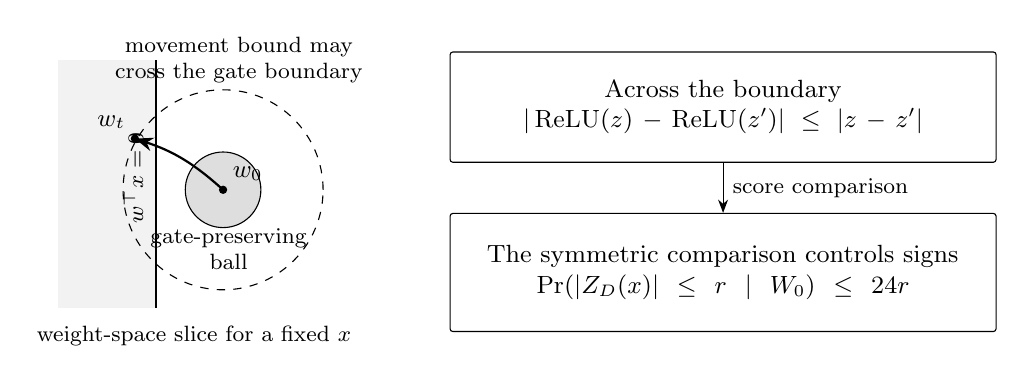
\begin{tikzpicture}[>=Stealth,font=\small]
 \begin{scope}
  \fill[black!5] (-1.25,-1.5) rectangle (0,1.65);
  \draw[thick] (0,-1.5)--(0,1.65);
  \node[rotate=90,anchor=south,font=\footnotesize] at (-0.04,0.15) {$w^\top x=0$};
  \fill[black!13] (0.85,0) circle (0.48);
  \draw (0.85,0) circle (0.48);
  \draw[dashed] (0.85,0) circle (1.27);
  \fill (0.85,0) circle (1.5pt);
  \node[above right] at (0.85,0) {$w_0$};
  \draw[->,thick] (0.85,0) to[bend right=12] (-0.27,0.65);
  \fill (-0.27,0.65) circle (1.5pt);
  \node[above left] at (-0.27,0.65) {$w_t$};
  \node[align=center,font=\footnotesize] at (0.92,-0.75) {gate-preserving\\ball};
  \node[align=center,font=\footnotesize] at (1.05,1.65) {movement bound may\\cross the gate boundary};
  \node[align=center,font=\footnotesize] at (0.48,-1.85) {weight-space slice for a fixed $x$};
 \end{scope}
 \node[draw,rounded corners=1pt,align=center,text width=67mm,minimum height=14mm] (score) at (7.2,1.05)
   {Across the boundary\\$|\relu(z)-\relu(z')|\le|z-z'|$};
 \node[draw,rounded corners=1pt,align=center,text width=67mm,minimum height=15mm] (null) at (7.2,-1.05)
   {The symmetric comparison controls signs\\$\Pr(|Z_D(x)|\le r\mid W_0)\le24r$};
 \draw[->] (score.south)--node[right,font=\footnotesize]{score comparison}(null.north);
\end{tikzpicture}
\caption{Gate stability is sufficient for exact frozen-gate identities, but the present score bound also controls crossings. The classification argument uses anti-concentration of a label-symmetric comparison score. The radius in this schematic is illustrative; the proof uses a Frobenius displacement bound for the entire input layer.}
\label{fig:gates}
\end{figure}

\section{Gate changes and parity}
The regime allows many activation changes at the test point itself. This separates the proof from an argument that discards all points at which any gate changes.

\begin{proposition}[First-step crossings at linear width]
\label{prop:crossings}
Fix $C_0\ge2^{20}$, an integer $T_0\ge2^{24}$, and $B\in(0,12]$. For each $n$, set $m_n=\lceil C_0n\rceil$ and $\eta_n=B/(m_nT_0)$. Choose any $x_n\in\X_n$ and train on its point mass with positive label. Let $N_n$ count rows for which
\[
 w_{0j}^\top x_n>0\quad\text{and}\quad w_{1j}^\top x_n<0.
\]
For every fixed integer $J$, $\Pr[N_n\ge J]\to1$ as $n\to\infty$. All these schedules satisfy \eqref{eq:regime}.
\end{proposition}

The kernel correlation also yields a direct obstruction for high-order parity. Under the uniform cube distribution, the Gaussian law makes every Fourier coefficient of a given degree have the same expected squared magnitude. Parseval's identity bounds their sum by $1/2$.

\begin{corollary}[Parity obstruction]
\label{cor:parity}
Under \eqref{eq:regime}, for every $A\subseteq[n]$ with $|A|=k$,
\begin{equation}
 \Risk(\chi_A,\Unif(\X_n))
 \ge\frac38-\frac{9B}{\sqrt{2\binom nk}},
 \qquad \chi_A(x)=\prod_{i\in A}x_i.
 \label{eq:parity}
\end{equation}
In particular, if $\binom nk>2592B^2$, the process cannot learn $\chi_A$ to expected error below $1/4$ under every marginal. This applies to the even half-size parity orbit when $n$ is divisible by four and sufficiently large.
\end{corollary}

\section{Scope}
The proof uses bounded effective time. Although its score comparison permits many gate crossings, it remains kernel-like and gives no feature-learning separation. The cutoff $B=12$ and the constants in \eqref{eq:regime} are sufficient conditions; they do not locate a transition for $B$ growing with $n$. Equation~\eqref{eq:risk-general} retains the quantitative losses.

The common representation is existential. The crossing proposition assumes no learning success; the ordinary-dimension theorem assumes \eqref{eq:premise}. The accompanying computations check proof formulas rather than convergence.

\begin{thebibliography}{9}
\bibitem[Allen-Zhu et~al.(2019)Allen-Zhu, Li, and Liang]{AllenZhu19}
Zeyuan Allen-Zhu, Yuanzhi Li, and Yingyu Liang.
\newblock Learning and generalization in overparameterized neural networks, going beyond two layers.
\newblock In \emph{Advances in Neural Information Processing Systems}, volume~32, 2019.
\newblock arXiv:1811.04918.

\bibitem[Chizat et~al.(2019)Chizat, Oyallon, and Bach]{Chizat19}
L\'ena\"ic Chizat, Edouard Oyallon, and Francis Bach.
\newblock On lazy training in differentiable programming.
\newblock In \emph{Advances in Neural Information Processing Systems}, volume~32, 2019.
\newblock arXiv:1812.07956.

\bibitem[Daniely(2017)]{Daniely17}
Amit Daniely.
\newblock SGD learns the conjugate kernel class of the network.
\newblock In \emph{Advances in Neural Information Processing Systems}, volume~30, 2017.
\newblock arXiv:1702.08503.

\bibitem[Feldman et~al.(2026)Feldman, Kamath, and Srebro]{FKS26}
Vitaly Feldman, Pritish Kamath, and Nathan Srebro.
\newblock Invited open problem: Is the power of deep learning over linear models inherently distribution dependent?
\newblock In \emph{Proceedings of the Thirty-Ninth Conference on Learning Theory}, volume~336 of \emph{Proceedings of Machine Learning Research}, pages 7117--7122, 2026.
\newblock \url{https://proceedings.mlr.press/v336/feldman26a.html}.

\bibitem[Ji and Telgarsky(2020)]{JiT20}
Ziwei Ji and Matus Telgarsky.
\newblock Polylogarithmic width suffices for gradient descent to achieve arbitrarily small test error with shallow ReLU networks.
\newblock In \emph{International Conference on Learning Representations}, 2020.
\newblock arXiv:1909.12292v4.

\bibitem[Kamath et~al.(2020)Kamath, Montasser, and Srebro]{KMS20}
Pritish Kamath, Omar Montasser, and Nathan Srebro.
\newblock Approximate is good enough: Probabilistic variants of dimensional and margin complexity.
\newblock In \emph{Proceedings of the Thirty-Third Conference on Learning Theory}, volume~125 of \emph{Proceedings of Machine Learning Research}, pages 2236--2262, 2020.
\newblock arXiv:2003.04180.

\bibitem[Malach et~al.(2021)Malach, Yehudai, Shalev-Shwartz, and Shamir]{Malach21}
Eran Malach, Gilad Yehudai, Shai Shalev-Shwartz, and Ohad Shamir.
\newblock The connection between approximation, depth separation and learnability in neural networks.
\newblock In \emph{Proceedings of the Thirty-Fourth Conference on Learning Theory}, volume~134 of \emph{Proceedings of Machine Learning Research}, pages 3265--3295, 2021.
\newblock \url{https://proceedings.mlr.press/v134/malach21a.html}.

\bibitem[Yehudai and Shamir(2020)]{Yehudai20}
Gilad Yehudai and Ohad Shamir.
\newblock Learning a single neuron with gradient methods.
\newblock In \emph{Proceedings of the Thirty-Third Conference on Learning Theory}, volume~125 of \emph{Proceedings of Machine Learning Research}, pages 3756--3786, 2020.
\newblock \url{https://proceedings.mlr.press/v125/yehudai20a.html}.
\end{thebibliography}

\clearpage
\appendix
\section{Uniform feature norms and the actual score comparison}
\label{app:comparison}
For the rest of the proof let $\lambda=7/16$, $\Lambda=9/16$, and $\psi(x)=m^{-1/2}\relu(W_0x)$. Define
\begin{equation}
 \Gcal=\{W_0:\lambda\le\norm{\psi(x)}^2\le\Lambda\text{ for every }x\in\X_n\}.
 \label{eq:good}
\end{equation}
The event is fixed before any target, marginal, or sample history is selected.

\begin{lemma}[Initialization bounds]
\label{lem:init}
The initialization satisfies
\[
 \Pr(W_0\notin\Gcal)\le\rho_W,
 \qquad \Pr(\norm{a_0}>2)\le\rho_a.
\]
\end{lemma}
\begin{proof}
Fix $x$. The variables $Y_j=\relu(w_{0j}^\top x)^2$ are independent with the law of $Y=Z^2\ind\{Z>0\}$ for $Z\sim N(0,1)$. Its mean is $1/2$ and
\[
 M(\theta)=\E e^{\theta Y}=\frac{1+(1-2\theta)^{-1/2}}2.
\]
For $|\theta|\le1/4$, $M\ge1/2$ and $M''\le(3/2)2^{5/2}$. Hence $(\log M)''\le32$. Since $(\log M)'(0)=1/2$, integration gives
\[
 \log\E e^{\theta(Y-1/2)}\le16\theta^2.
\]
Apply Chernoff's inequality with $\theta=\pm1/512$. Each tail at distance $1/16$ from the mean has probability at most $e^{-m/16384}$. The union bound over $2^n$ points proves the first claim. This is the only union bound over the cube in the argument.

Also $m\norm{a_0}^2$ has the $\chi_m^2$ law. Markov's inequality applied to $e^{\chi_m^2/4}$ gives
\[
 \Pr(\norm{a_0}>2)\le e^{-m}2^{m/2}\le e^{-m/2}.
\]
\end{proof}

Put $g(y,z)=y/(1+e^{yz})$. It has absolute value at most one and derivative in $z$ between $-1/4$ and zero. On any labeled history, introduce a linear comparison $u_t$ by
\begin{equation}
 u_0=\sqrt m\,a_0,
 \qquad
 u_{t+1}=u_t+\gamma g(y_t,u_t^\top\psi(x_t))\psi(x_t),
 \qquad \gamma=\eta m.
 \label{eq:frozen}
\end{equation}
This is an auxiliary recurrence using the same samples. It is used only to estimate the stipulated trajectory.

\begin{lemma}[Score comparison through gate changes]
\label{lem:score}
Suppose $W_0\in\Gcal$, $\norm{a_0}\le2$, $m\ge576n$, $B\le12$, and $\gamma\le1/2$. For every labeled history,
\begin{equation}
 \max_{0\le t\le T}\max_{x\in\X_n}
   |f_t(x)-u_t^\top\psi(x)|\le\kappa=544n/m.
 \label{eq:score-compare}
\end{equation}
The same bound holds for the normalized tail scores.
\end{lemma}
\begin{proof}
Write
\[
 A=\max_{t\le T}\norm{a_t},\qquad
 D_W=\max_{t\le T}\norm{W_t-W_0}_F.
\]
These quantities are finite for every finite initialization and finite history. From the actual input-layer updates,
\begin{equation}
 D_W\le\eta T\sqrt n\, A=\frac{B\sqrt n}{m}A.
 \label{eq:DW}
\end{equation}
ReLU is 1-Lipschitz, so
\[
 \norm{\relu(W_tx)}\le\sqrt{m\Lambda}+\sqrt n\,D_W.
\]
Summing the output-layer increments and using \eqref{eq:DW} yields
\[
 A\le\norm{a_0}+B\sqrt{\Lambda/m}+\frac{B^2n}{m^2}A.
\]
Under the hypotheses, $B^2n/m^2\le1/4$ and $B\sqrt{\Lambda/m}\le3/8$. Thus $A<4$ and $D_W\le4B\sqrt n/m$.

Let $b_t=\sqrt m\,a_t$ and define
\[
 e_t(x)=m^{-1/2}\bigl(\relu(W_tx)-\relu(W_0x)\bigr),
 \qquad r_t(x)=f_t(x)-b_t^\top\psi(x).
\]
Uniformly in $t,x$,
\begin{equation}
 \norm{e_t(x)}\le e_*:=\frac{4Bn}{m^{3/2}},
 \qquad |r_t(x)|\le r_*:=\frac{16Bn}{m}.
 \label{eq:residuals}
\end{equation}
These estimates use no gate-sign assertion.

For fixed $(x,y)$, the map $S_{x,y}(v)=v+\gamma g(y,v^\top\psi(x))\psi(x)$ has derivative $I-\gamma\ell''\psi(x)\psi(x)^\top$, where $0\le\ell''\le1/4$. As $\gamma\le1/2$ and $\norm{\psi(x)}^2\le\Lambda$, this derivative is positive semidefinite with operator norm at most one. Hence $S_{x,y}$ is nonexpansive. Comparing the exact update of $b_t$ with $S_{x_t,y_t}(b_t)$ gives a residual of norm at most
\[
 \gamma\bigl(\sqrt\Lambda\,r_*/4+e_*\bigr).
\]
Iterating nonexpansivity from $b_0=u_0$ proves
\[
 \norm{b_t-u_t}\le B\bigl(\sqrt\Lambda\,r_*/4+e_*\bigr).
\]
Consequently,
\[
 |f_t(x)-u_t^\top\psi(x)|
 \le(1+B\Lambda/4)r_*+B\sqrt\Lambda\,e_*.
\]
The first term is at most $516n/m$. The second is at most $432n/m^{3/2}\le18n/m$, since $m\ge576$. Their sum is at most $544n/m$. Averaging the scores over $I_T$ preserves the bound.
\end{proof}

\section{Population comparison and Gaussian anti-concentration}
\label{app:null}
Fix $W_0\in\Gcal$, a Boolean target $h$, and a marginal $D$. Let
\[
 \mu=\E_D h(x)\psi(x),\qquad
 R(v)=v-\frac\gamma2\E_D\left[\psi(x)\tanh\bigl(v^\top\psi(x)/2\bigr)\right].
\]
The map $R$ is odd. Its derivative is
\begin{equation}
 DR(v)=I-\gamma H(v),\qquad
 H(v)=\frac14\E_D\left[\psi(x)\psi(x)^\top
             \operatorname{sech}^2\bigl(v^\top\psi(x)/2\bigr)\right],
 \label{eq:H}
\end{equation}
and $0\preceq H(v)\preceq(\Lambda/4)I$. Both $R$ and $R+\gamma\mu/2$ are nonexpansive when $\gamma\le1/2$.

With the same initial $b_0=\sqrt m\,a_0$, define the population and symmetric recurrences
\begin{equation}
 v_0=z_0=b_0,
 \qquad v_{t+1}=R(v_t)+\gamma\mu/2,
 \qquad z_{t+1}=R(z_t).
 \label{eq:population}
\end{equation}
They are mathematical comparisons, and require no modification of \eqref{eq:actual}.

\begin{lemma}[Sampling and label effects]
\label{lem:population}
Conditionally on $W_0,b_0$,
\begin{equation}
 \E\norm{u_t-v_t}^2\le t\gamma^2\Lambda.
 \label{eq:samplevariance}
\end{equation}
For every $b_0$,
\begin{equation}
 \norm{v_t-z_t}\le t\gamma\norm\mu/2.
 \label{eq:labeldifference}
\end{equation}
In particular, if $\bar u=q^{-1}\sum_{t\in I_T}u_t$ and similarly for $\bar v,\bar z$, then
\begin{equation}
 \Pr(\norm{\bar u-\bar v}>u\mid W_0,b_0)
 \le\frac{\Lambda B^2}{Tu^2},
 \qquad
 |\ip{\bar v-\bar z}{\psi(x)}|\le\frac{3B}{8}\norm\mu.
 \label{eq:tailcomparisons}
\end{equation}
\end{lemma}
\begin{proof}
Let $P=R+\gamma\mu/2$. Given the past, the sample update \eqref{eq:frozen} has conditional mean $P(u_t)$. Write it as $P(u_t)+\gamma\xi_t$, where $\E[\xi_t\mid\text{past}]=0$ and
\[
 \E[\norm{\xi_t}^2\mid\text{past}]
 \le\E_D\norm{g(h(x),u_t^\top\psi(x))\psi(x)}^2\le\Lambda.
\]
The cross term vanishes in the conditional second moment. Nonexpansivity of $P$ therefore gives
\[
 \E[\norm{u_{t+1}-v_{t+1}}^2\mid\text{past}]
 \le\norm{u_t-v_t}^2+\gamma^2\Lambda.
\]
Induction proves \eqref{eq:samplevariance}. Nonexpansivity of $R$ gives
$\norm{v_{t+1}-z_{t+1}}\le\norm{v_t-z_t}+\gamma\norm\mu/2$, proving \eqref{eq:labeldifference}. Jensen's inequality for the tail average and Markov's inequality give the first assertion of \eqref{eq:tailcomparisons}. The second uses $\norm{\psi(x)}\le\sqrt\Lambda=3/4$.
\end{proof}

\begin{lemma}[Density at the beginning of the tail]
\label{lem:density}
Assume $W_0\in\Gcal$, $B\le12$, and $\gamma\le1/2$. Put $s=\lceil T/2\rceil$. The law of $z_s$, conditional on $W_0$, has a density $q_s$ satisfying
\begin{equation}
 q_s(v)\le e\,(2\pi)^{-m/2}\exp(-\norm v^2/2).
 \label{eq:density}
\end{equation}
\end{lemma}
\begin{proof}
Besides the operator bound in \eqref{eq:H}, we have $\operatorname{tr}H(v)\le\Lambda/4$. Let $a=\gamma\Lambda/4<1$. Every eigenvalue of $DR(v)$ lies in $[1-a,1]$. The map $R$ is a global smooth diffeomorphism. Indeed, it is the gradient of
\[
 U(v)=\tfrac12\norm v^2-\gamma\E_D\log\cosh(v^\top\psi(x)/2),
\]
whose Hessian is at least $(1-a)I$. Subtracting any linear functional leaves a strongly convex, coercive function, whose unique minimizer solves the corresponding inverse equation. Strong monotonicity proves injectivity, and the inverse function theorem supplies smoothness.

For $0\le t\le a$, $-\log(1-t)\le t/(1-a)$. Thus
\[
 -\log\det DR(v)\le\frac{\gamma\operatorname{tr}H(v)}{1-a}
 \le\frac{\gamma\Lambda}{4(1-a)}.
\]
The same determinant bound multiplies over the $s$ steps. Since $R$ is nonexpansive and fixes zero, its inverse trajectory satisfies $\norm{b_0}\ge\norm{z_s}$. Change of variables from the standard Gaussian $b_0$ therefore yields
\[
 q_s(v)\le\exp\left(\frac{s\gamma\Lambda}{4(1-\gamma\Lambda/4)}\right)
            (2\pi)^{-m/2}e^{-\norm v^2/2}.
\]
Here $s\gamma\le B/2+\gamma/2\le25/4$. With $\gamma\le1/2$ and $\Lambda=9/16$, the exponent is at most $225/238<1$. This proves \eqref{eq:density}. The trace bound, rather than an $m$-dimensional operator-norm determinant bound, keeps the factor independent of width.
\end{proof}

\begin{lemma}[Anti-concentration of the symmetric tail]
\label{lem:smallball}
Assume $W_0\in\Gcal$, $B\le12$, and $\gamma\le1/2$. For each $x\in\X_n$, let
\[
 Z_D(x;b_0)=\ip{\bar z(b_0)}{\psi(x)},\qquad b_0\sim N(0,I_m).
\]
For every $r\ge0$,
\begin{equation}
 \Pr_{b_0}(|Z_D(x;b_0)|\le r\mid W_0)\le24r.
 \label{eq:smallball}
\end{equation}
The law is symmetric and has no atom at zero. Hence, for every Boolean $h$,
\begin{equation}
 \E_{b_0}\err_D(\sgn Z_D(\cdot;b_0),h)=1/2.
 \label{eq:nullrisk}
\end{equation}
\end{lemma}
\begin{proof}
Put $s=\lceil T/2\rceil$ and $L=T-s$. Regard the tail as a function of $v=z_s$. Write $z^{[v]}_0=v$ and $z^{[v]}_{j+1}=R(z^{[v]}_j)$ for $0\le j<L$. Its Jacobians $J_j=D_vz^{[v]}_j$ obey
\[
 J_0=I,\qquad J_{j+1}=(I-\gamma H(z^{[v]}_j))J_j.
\]
Each factor is a contraction, so $\norm{J_j}_{\op}\le1$. Summing
$J_{j+1}-J_j=-\gamma H(z^{[v]}_j)J_j$ gives
\begin{equation}
 \norm{J_j-I}_{\op}\le j\gamma\Lambda/4
       \le B\Lambda/8\le27/32.
 \label{eq:Jac}
\end{equation}
No commutativity or symmetry of the product $J_j$ is asserted.

First give $v$ a standard Gaussian law, rather than its actual law. For fixed $x$, put $e_x=\psi(x)/\norm{\psi(x)}$ and decompose $v=ae_x+v_\perp$. Conditionally on $v_\perp$, $a$ is an independent standard Gaussian. At every $a,v_\perp$,
\begin{align}
 \frac{d}{da}\left[\frac1{L+1}\sum_{j=0}^L
             \ip{z^{[v]}_j}{\psi(x)}\right]
 &=\norm{\psi(x)}\,e_x^\top
     \left(\frac1{L+1}\sum_{j=0}^L J_j\right)e_x\notag\\
 &\ge\sqrt\lambda\,(1-B\Lambda/8)
 \ge\frac{5\sqrt7}{128}.
 \label{eq:derivative}
\end{align}
The inverse image of $[-r,r]$ has length at most $256r/(5\sqrt7)$. The maximum one-dimensional Gaussian density therefore gives a probability at most
\[
 \frac{256r}{5\sqrt{14\pi}}<8r.
\]
Lemma~\ref{lem:density} bounds the actual density of $z_s$ by $e$ times this Gaussian density. Consequently the actual small-ball probability is at most $8er<24r$.

The recurrence $R$ is odd, so $Z_D(x;-b_0)=-Z_D(x;b_0)$. The small-ball estimate excludes an atom at zero. Symmetry then proves error $1/2$ at every fixed test point, and averaging over $D$ proves \eqref{eq:nullrisk}.
\end{proof}

\section{From risk to a common kernel margin}
\label{app:margin}
\begin{proof}[Proof of Theorem~\ref{thm:risk}]
Fix $h,D$ before initialization, and condition on $W_0\in\Gcal$. For a test point $x$, put
\[
 Z=Z_D(x;b_0),\qquad
 d=\kappa+\frac{3B}{8}\norm\mu,\qquad
 E_x=\ip{\bar u-\bar v}{\psi(x)}.
\]
Lemmas~\ref{lem:score} and~\ref{lem:population} show that on $\{\norm{a_0}\le2\}$,
\[
 |F(x)-Z|\le d+|E_x|,\qquad
 \E[|E_x|^2\mid W_0,b_0]\le\sigma^2:=\frac{\Lambda^2 B^2}{T}.
\]
The second inequality is conditional on every $b_0$, which allows us to integrate the error probability against the Gaussian initialization without asserting independence of $E_x$ and $Z$.

Conditionally on $b_0$, when $|Z|>d$, Markov's inequality bounds the probability of a classification disagreement by
$\min\{1,\sigma^2/(|Z|-d)^2\}$, apart from the event $\norm{a_0}>2$. Give this minimum the value one when $|Z|\le d$. Its initialization expectation is, by the layer-cake identity and Lemma~\ref{lem:smallball}, at most
\begin{align*}
 \int_0^1\Pr_{b_0}\left(|Z|\le d+\frac{\sigma}{\sqrt t}\,\middle|\,W_0\right)dt
 &\le24\int_0^1\left(d+\frac{\sigma}{\sqrt t}\right)dt\\
 &=24d+48\sigma.
\end{align*}
The null classifier has expected error $1/2$. Average over the fixed test marginal and subtract the output-norm failure probability to obtain
\[
 \E[\err_D(G,h)\mid W_0]
 \ge\frac12-\rho_a-24\kappa-\frac{27B}{\sqrt T}-9B\norm\mu.
\]
The Gaussian small-ball calculation uses the unrestricted law of $b_0$; we have subtracted the output-norm failure event rather than conditioning that law on a ball.

For initializations outside $\Gcal$, retain only the nonnegativity of risk. After averaging,
\[
 \Risk(h,D)\ge\frac12(1-\rho_W)-\rho_a-24\kappa-\frac{27B}{\sqrt T}
       -9B\E[\ind_{\Gcal}\norm\mu].
\]
Independence and identical distribution of the hidden rows give the exact identity
\begin{align}
 \E_{W_0}\norm\mu^2
 &=\frac1m\sum_{j=1}^m\E_{w_{0j}}
       \left(\E_Dh(x)\relu(w_{0j}^\top x)\right)^2\notag\\
 &=A_D(h)^2.
 \label{eq:kernelidentity}
\end{align}
Thus $\E[\ind_{\Gcal}\norm\mu]\le A_D(h)$ by Cauchy--Schwarz. This proves \eqref{eq:risk-general}.

For \eqref{eq:risk-simple}, under \eqref{eq:regime} we have $\rho_W,\rho_a\le1/64$, and
\[
 \frac{27B}{\sqrt T}\le\frac{324}{4096},\qquad
 24\kappa\le\frac{51}{4096}.
\]
Including $\rho_W/2\le32/4096$ and $\rho_a\le64/4096$, the total loss is at most $471/4096<1/8$. Substitution proves \eqref{eq:risk-simple}.
\end{proof}

Suppose now that \eqref{eq:premise} holds. The last theorem implies
\begin{equation}
 \forall h\in\Hc\ \forall D\in\Delta(\X_n),\qquad
 \left\|\E_Dh(x)\Phi(x)\right\|_{\Kc}\ge c:=\frac1{72B}.
 \label{eq:allmarginal}
\end{equation}
The next elementary argument is where the all-marginal quantifier is used to obtain an exact representation.

\begin{lemma}[Convex separation and ordinary dimension]
\label{lem:geometry}
Let $X$ be a finite set of size $M\ge2$, let $\Phi:X\to\Kc$ have $\norm{\Phi(x)}^2\le1/2$, and suppose a nonempty Boolean class $\Hc$ satisfies \eqref{eq:allmarginal} with some $c>0$. Then every $h$ has a unit vector $u_h$ with $h(x)\ip{u_h}{\Phi(x)}\ge c$ for all $x$. In addition,
\[
 \VC(\Hc)\le\frac1{2c^2},\qquad
 \dc(\Hc)\le C c^{-2}(1+c^{-2})\log(2M)
\]
for a universal $C$.
\end{lemma}
\begin{proof}
For fixed $h$, the convex hull
\[
 C_h=\operatorname{conv}\{h(x)\Phi(x):x\in X\}
\]
is compact in a finite-dimensional subspace. Its elements are exactly the vectors $\E_Dh(x)\Phi(x)$. Let $p_h$ be its nearest point to zero. By the hypothesis, $\norm{p_h}\ge c$. Minimizing the squared norm along the segment from $p_h$ to any $z\in C_h$ gives
\[
 \ip{p_h}{z-p_h}\ge0.
\]
Thus $u_h=p_h/\norm{p_h}$ satisfies the stated margin on every point. In particular, $u_h$ depends on $h$ but not on $D$.

Suppose $r$ points are shattered. For every sign vector $\sigma\in\{-1,1\}^r$, a unit vector realizing its margins gives
\[
 rc\le\left\|\sum_{i=1}^r\sigma_i\Phi(x_i)\right\|.
\]
Average over independent fair signs and use the second moment to obtain $rc\le\sqrt{r/2}$. Hence $r\le1/(2c^2)$. With $v=\lceil1/(2c^2)\rceil\ge1$, the standard growth recursion, splitting a class according to its value on one point, gives
\[
 |\Hc|\le\sum_{i=0}^{\min(v,M)}\binom Mi\le(M+1)^v.
\]
The recursion is $N(M,v)\le N(M-1,v)+N(M-1,v-1)$: labelings that occur with both labels at the last point have VC dimension at most $v-1$ on the remaining points. Induction gives the displayed binomial bound.

It remains to project the finite collection of input and target vectors. All of them lie in the span of $\Phi(X)$, so choose an orthonormal basis there. A matrix with independent $N(0,1/d)$ entries gives, for each fixed vector $z$ and $0<a<1$,
\[
 \Pr\left(\big|\norm{Jz}^2-\norm z^2\big|>a\norm z^2\right)
 \le2e^{-da^2/8}.
\]
This is the elementary chi-square Chernoff bound. Apply it to $u_h+\Phi(x)$ and $u_h-\Phi(x)$ for all $h,x$, with $a=c/2$. A sufficiently large
\[
 d\le C c^{-2}\log\bigl(4|\Hc|M\bigr)
\]
permits a realization preserving all these squared norms to relative error $a$. Polarization bounds each inner-product error by
\[
 \frac a2\bigl(\norm{u_h}^2+\norm{\Phi(x)}^2\bigr)
 \le\frac{3c}{8}<\frac c2.
\]
Thus $J\Phi(x)$ and $Ju_h$ strictly represent the truth table. If this dimension exceeds the finite span dimension, use the identity map instead. The growth bound above gives the stated estimate. Nonemptiness implies $c\le1/\sqrt2$, so the choice $a=c/2$ is valid.
\end{proof}

\begin{proof}[Proof of Theorem~\ref{thm:ordinary}]
Apply Lemma~\ref{lem:geometry} to \eqref{eq:allmarginal}, with $M=2^n$ and $c=1/(72B)$. This gives the kernel margin and $\VC(\Hc)\le2592B^2$. Its dimension bound is at most $C(1+B)^4(n+1)$ after changing a universal constant. Since $B\le12$, a further universal constant gives the final bound in \eqref{eq:ordinarybound}. The empty class is immediate.
\end{proof}

\section{Proofs of the crossing and parity statements}
\label{app:consequences}
\begin{proof}[Proof of Proposition~\ref{prop:crossings}]
Write $z_j=w_{0j}^\top x_n$ and $b_j=\sqrt m\,a_{0j}$. The pairs $(z_j,b_j)$ are independent standard Gaussian pairs. The initial score
\[
 f_0(x_n)=m^{-1/2}\sum_j b_j\relu(z_j)
\]
has mean zero and variance $1/2$, for every $n,m$.

Fix $R>0$. On $\{f_0(x_n)\le R\}$, an initially active row updates according to
\[
 w_{1j}^\top x_n=z_j+\frac{\eta_n n\,b_j}{\sqrt m(1+e^{f_0(x_n)})}.
\]
It becomes strictly negative whenever
\[
 b_j\le-1,\qquad 0<z_j<d_n,
 \qquad d_n=\frac{\eta_n n}{\sqrt m(1+e^R)}.
\]
Let $C_n$ count these candidate rows. It is binomial, and
\[
 \E C_n=m\Pr(b_j\le-1)\Pr(0<z_j<d_n)
 \asymp_R\frac{B n}{T_0\sqrt m}\longrightarrow\infty.
\]
Here $m=\lceil C_0n\rceil$, $d_n\to0$, and $B,C_0,T_0,R$ are fixed. Therefore $\Pr(C_n<J)\to0$ for every fixed $J$. No independence between $C_n$ and the initial score is required: the union bound and the score's variance give
\[
 \Pr(N_n<J)\le\Pr(C_n<J)+\Pr(f_0(x_n)>R)
 \le\Pr(C_n<J)+\frac1{2R^2}.
\]
Take the upper limit in $n$, then let $R\to\infty$. All computations use the old output coefficient, as required by simultaneous SGD.
\end{proof}

\begin{proof}[Proof of Corollary~\ref{cor:parity}]
For each $w$, let $\widehat r_w(A)=\E_{x\sim\Unif(\X_n)}\chi_A(x)\relu(w^\top x)$. Coordinate-permutation invariance of the Gaussian law implies that
\[
 \lambda_k=\E_w\widehat r_w(A)^2
\]
depends only on $|A|=k$. Parseval's identity and nonnegativity give
\[
 \binom nk\lambda_k
 \le\sum_{A\subseteq[n]}\E_w\widehat r_w(A)^2
 =\E_w\E_x\relu(w^\top x)^2=\frac12.
\]
But $A_D(\chi_A)^2=\lambda_k$ for the uniform marginal. Substitute in \eqref{eq:risk-simple}. The bound exceeds $1/4$ whenever $\binom nk>2592B^2$, which proves the failure of the all-marginal guarantee.
\end{proof}

\end{document}
